\documentclass[12pt]{report}

\usepackage[a4paper, total={17cm, 24cm}]{geometry}
\usepackage{exercise}

\renewcommand{\ExerciseHeader}{\noindent\textbf{\large\ExerciseName\ %
		\ExerciseHeaderNB\ExerciseHeaderTitle
		\ExerciseHeaderOrigin\medskip}}
\setlength{\QuestionIndent}{1.5em}

\newcommand{\answerbox}[2]{\hfill\break\\
	\framebox[\linewidth]{\parbox[c][#1][c]{\dimexpr\linewidth-2\fboxsep-2\fboxrule}{#2}}
}

\renewcommand{\arraystretch}{1.2} % vertical padding for tabular environment

% taken from https://texample.net/tikz/examples/sudoku/
\usepackage{tikz}
\usepackage{mathpazo}
\newcounter{row}
\newcounter{col}
\usepackage{graphicx}

\newcommand\setrowthree[3]{
	\setcounter{col}{1}
	\foreach \n in {#1, #2, #3} {
		\edef\x{\value{col} - 0.5}
		\edef\y{3.5 - \value{row}}
		\node[anchor=center] at (\x, \y) {\n};
		\stepcounter{col}
	}
	\stepcounter{row}
}

\newcommand\setrowfour[4]{
	\setcounter{col}{1}
	\foreach \n in {#1, #2, #3, #4} {
		\edef\x{\value{col} - 0.5}
		\edef\y{4.5 - \value{row}}
		\node[anchor=center] at (\x, \y) {\n};
		\stepcounter{col}
	}
	\stepcounter{row}
}

\begin{document}

	\hfill
	\begingroup
	\Large
	\begin{tabular}{|l|p{6cm}|}
		\hline
		First \& last name &
		% YOUR NAME HERE
		\\ \hline
		NOMA UCLouvain &
		% YOUR NOMA HERE
		\\ \hline
	\end{tabular}
	\endgroup
	\vspace{1.5cm}

	\noindent
	\begingroup
	\Large
	\textbf{LINFO2266: Advanced Algorithms for Optimization}\\\\
	Project 5: Constraint Programming
	\endgroup
	\vspace{0.2cm}

	\begin{Exercise}[title={Modeling the Magic Square Problem}]

		The Magic Square Problem is a famous combinatorial optimization problem where a square of $n\times n$ cells has to be filled such that all rows, columns and both diagonals sum to the same value and such that each number $i \in 1..n^2$ appears exactly once within the square.

		This problem can be modeled in constraint programming by applying 2 types of constraints on the variables representing the problem: \texttt{NotEqual} and \texttt{Sum} constraints.

		\Question What is the minimum number of variables needed to represent the problem?
		\answerbox{2cm}{
			% YOUR ANSWER HERE
		}

		\Question What is the minimum number of \texttt{NotEqual} and \texttt{Sum} constraints that needs to be applied on the problem to have a valid model? Give the number of times each type of constraint appears.
		\answerbox{3cm}{
			% YOUR ANSWER HERE
		}

		\Question The sum of each row, column and of both diagonal must be the same. What is the value of this sum for a $n\times n$ magic square? How can you derive it?
		\answerbox{4cm}{
			% YOUR ANSWER HERE
		}

		In the Magic Square Problem, we are interested in counting the number of solutions that exist. However, some symmetrical solutions can be easily found once you have one. For instance, given the following magic square solution (left), you can derive the other one (right) by applying some kind of transformation.

		\begin{minipage}{0.4\linewidth}
			\centering
			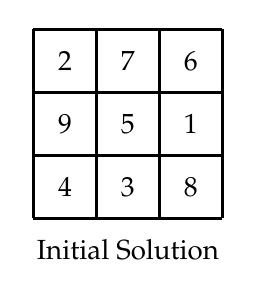
\begin{tikzpicture}[scale=0.8]

				\begin{scope}
					\draw (0, 0) grid (3, 3);
					\draw[very thick] (0, 0) grid (3, 3);

					\setcounter{row}{1}
					\setrowthree {2}{7}{6}
					\setrowthree {9}{5}{1}
					\setrowthree {4}{3}{8}
					\node[anchor=center] at (1.5, -0.5) {Initial Solution};
				\end{scope}
			\end{tikzpicture}
		\end{minipage}
		\hfill
		\begin{minipage}{0.4\linewidth}
			\centering
			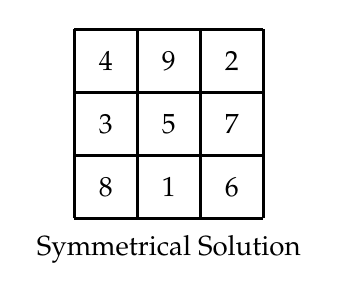
\begin{tikzpicture}[scale=0.8]

				\begin{scope}
					\draw (0, 0) grid (3, 3);
					\draw[very thick] (0, 0) grid (3, 3);

					\setcounter{row}{1}
					\setrowthree {4}{9}{2}
					\setrowthree {3}{5}{7}
					\setrowthree {8}{1}{6}
					\node[anchor=center] at (1.5, -0.5) {Symmetrical Solution};
				\end{scope}
			\end{tikzpicture}
		\end{minipage}

		\Question Given the following magic square solution, how many symmetrical solutions can you derive from it? What are the operations that you can apply to find them?

		\begin{center}
			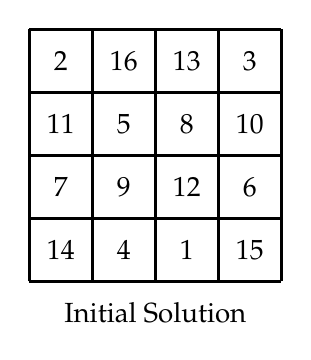
\begin{tikzpicture}[scale=0.8]

				\begin{scope}
					\draw (0, 0) grid (4, 4);
					\draw[very thick] (0, 0) grid (4, 4);

					\setcounter{row}{1}
					\setrowfour {2}{16}{13}{3}
					\setrowfour {11}{5}{8}{10}
					\setrowfour {7}{9}{12}{6}
					\setrowfour {14}{4}{1}{15}
					\node[anchor=center] at (2, -0.5) {Initial Solution};
				\end{scope}
			\end{tikzpicture}
		\end{center}


		\answerbox{12cm}{
			% YOUR ANSWER HERE
		}

		\Question Use your solver to solve a magic square of size $4\times4$ cells, without any cell with an initial value (i.e. all values are unknown). Report the number of solutions found, the number of failures encountered and the number of recursive calls to the method \texttt{dfs} when looking for all solutions to the instance.

		\answerbox{2cm}{
			% YOUR ANSWER HERE
		}

		\Question Experiment with symmetry breaking. For the same instance as in the previous question, experiment with the two following situations:
		\begin{enumerate}
			\item find all solutions to the instance ;
			\item add first a constraint $cell[0][0] \leq cell[0][1]$ to break some symmetrical solutions. Then, find all solutions to the instance.
		\end{enumerate}
		Plot the number of solutions found over time in the two scenarios. The x-axis must be the time elapsed, in seconds. The y-axis must be the total number of solutions encountered so far.

		\answerbox{10cm}{
			% YOUR ANSWER HERE
		}

	\end{Exercise}

	\pagebreak

	\begin{Exercise}[title={Knight Tour}]

		In the Knight Tour problem, we have chosen a model
		where the $x[i]$ is the position visited in step $i$.
		An alternative \textit{successor} model is to use $x[i]$ as a variable representing
		the next position after having visited the position $i$.
		\Question Discuss the advantages and inconvenients of each modeling approach with respect 
		to the number of symmetrical solutions that are generated?
		\answerbox{6cm}{
			% YOUR ANSWER HERE
		}
		\Question How would you enforce the valid knight moves using the successor model?
		\answerbox{7cm}{
			% YOUR ANSWER HERE
		}

	\end{Exercise}

\end{document}